\documentclass{beamer}
%\documentclass[notes=only]{beamer}   % only notes
\usetheme[progressbar=foot]{metropolis}

\setbeamertemplate{frame footer}{\tiny{ \inserttitle \, \textbar\,  \insertauthor \, \textbar \,  \insertdate}}

% IMPORTS
\usepackage[ngerman]{babel}
\usepackage[utf8]{inputenc}
% \usepackage[T1]{fontenc}
\usepackage{graphicx}	% Einbinden von Grafiken
\usepackage{float}		% figure: [H]
\usepackage{wrapfig}	% figure: [l]
\usepackage{subfigure}
\usepackage{caption}
\usepackage{url}
\usepackage{hyperref}
\usepackage{hepnames}
\usepackage{csquotes}
\usepackage[style=numeric,backend=biber]{biblatex}


% Set bib file
\bibliography{literature}

% Removes icon in bibliography
\setbeamertemplate{bibliography item}{}

% Custom colors
\usepackage{xcolor}
\definecolor{deepblue}{RGB}{46,206,227}
\definecolor{deepred}{RGB}{245,20,66}
\definecolor{deepgreen}{RGB}{98,213,51}
\definecolor{deepgrey}{RGB}{183,183,183}
\definecolor{deepyellow}{RGB}{222,203,80}
\definecolor{commentgreen}{RGB}{78,139,70}

\usepackage{listings}

\lstset{ 
language=Python,
basicstyle=\fontsize{9}{9}\ttfamily,
otherkeywords={self},                   % Add keywords here
keywordstyle=\ttfamily\color{deepblue},
emph={MyClass,__init__},                % Custom highlighting
emphstyle=\ttfamily\color{deepred},     % Custom highlighting style
stringstyle=\color{deepgreen},
commentstyle=\color{commentgreen},      % comment style
frame=trbl,                             % Any extra options here
tabsize=4,
showstringspaces=false,
breaklines=true,
numbers=left,
extendedchars=false,
mathescape=true,
escapeinside={(*}{*)},
literate=%
    {ä}{{\"a}}1
    {ö}{{\"o}}1
    {ü}{{\"u}}1
    {ß}{{\ss}}1
}

\title{Grundkurs: Programmieren}
\subtitle{Einführung in grundlegende Programmierkonzepte mit Python}
\date{ WS 18/19 }
\author[CS]{ Maren Krafft }
\institute{ Universität Passau }
\subject{Computer Science}

\begin{document}
\maketitle

\section{Einführung in die Programmierung}

\begin{frame}{Vorstellung}
\begin{itemize}
	\item Name
	\item Studiengang 
	\item Programmiererfahrung allgemein
	\item Programmiererfahrung Python
	\item Erwartungen
\end{itemize}
\end{frame}

\begin{frame}{Organisatorisches}
    \begin{itemize}
        \item Anwesenheitspflicht
        \item Teilnahmebestätigung (Zertifikat)
        \item "Regeln"
        \item Codio
        \item Skript
    \end{itemize}
\end{frame}

\begin{frame}{Ablauf}
\begin{tabular}{ l l }
	14.00 - 14.15 & Erwartungen und Vorkenntnisse\\
	14.15 - 14.45 & Einführung in Python und Umgebung \\
	14.45 - 15.30 & Datentypen, Operatoren, Variablen und Zuweisungen\\
	15.30 - 15.45 & Pause \\
	15.45 - 16.45 & Bedingte Ausführung \\
	17.00 - 18.00 & Schleifen \\
	
\end{tabular}
\end{frame}

\begin{frame}{Ablauf}

\begin{tabular}{ l l }
	10.15 - 10.30 & Besprechung Tagesplan\\
	10.30 - 11.30 & Wiederholung \\
	11.30 - 12.30 & Typconventionen\\
	11.00 - 11.30 & Funktionen \\
	11.30 - 11.45 & Pause\\
	11.45 - 12.00 & Listen\\
	13.00 - 13.45 & Mittagspause\\
	13.45 - 15.30 & Datein einlesen/ausgeben\\
	15.30 - 16.00 & allgemeine Theorie\\
	
\end{tabular}
\end{frame}

\begin{frame}{Die Programmiersprache Python}
\begin{columns}
    \column{0.5\textwidth}
    \begin{itemize}
        \item Warum Python?
            \begin{itemize}
                \item flache Lernkurve, sehenswerte Ergebnisse bereits nach dem ersten Tag
                \item verankert in Forschung und Wirtschaft
                \item der englischen Sprache sehr änhlich
            \end{itemize}
    \end{itemize}
    \column{0.5\textwidth}
    \centering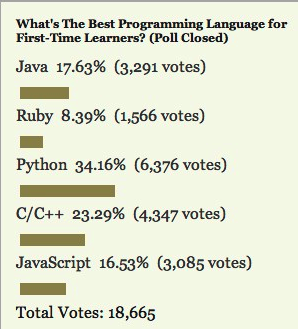
\includegraphics[scale=0.5]{images/best_lang} 
    \hyperlink{https://lifehacker.com/five-best-programming-languages-for-first-time-learners-1494256243}{\tiny{Quelle: lifehacker.com}}
\end{columns}
\end{frame}


\section{Codio}


\begin{frame}[fragile]{Allgemeines zu Python}
Kommentare
\begin{itemize}
	\item Wir kommentieren mit \#
	
	\begin{lstlisting}
	# Einfach so
	\end{lstlisting}

	\item Einzeiler
	\item Sinnvolle Kommentare
\end{itemize}
\end{frame}

\begin{frame}{Programm/Sequenz}
Programm
\begin{itemize}
	\item wird "von oben nach unten" ausgeführt
\end{itemize}
\end{frame}

\begin{frame}{Funktion}
	\begin{itemize}
	\item wird ähnlich wie in der Mathematik verwendet (nur nicht mit Zahlen)
	\item eine Vielzahl von Befehlen (vorgefertigt oder selbstgeschrieben) zusammengefasst in einer bestimmten Schreibweise	
	\end{itemize}
\end{frame}
\section{Datentypen}

\begin{frame}[fragile]{Datentypen}
Lernziele
\begin{itemize}
	\item Die wichtigsten Datentypen kennenlernen
	\item Diese ausgeben können
	\item Datentypen in andere Datentypen umwandeln
\end{itemize}
\end{frame}

\begin{frame}[fragile]{Erste wichtige Funktion: print()}

	Gibt alles innerhalb den Klammern auf die Konsole aus.

\begin{lstlisting}
print("Hallo")
print(1)
print(1+2)
\end{lstlisting}
\end{frame}



%Einführung String
\begin{frame}[fragile]{String}
\begin{itemize}
    \item \texttt{String, str}: 
     	\begin{itemize}
     		\item ist eine Zeichenkette
     		\item wird in '' '' geschrieben
     	\end{itemize}
     \end{itemize}
    \begin{lstlisting}
"Ich bin vom Typ String, eine Reihe von Zeichen"
"1"
" "
    \end{lstlisting}
\end{frame}

%Beispielaufgabe für String
\begin{frame}[fragile]{Hello World}
\begin{lstlisting}
print("Hello World!")
\end{lstlisting}
\begin{itemize}
	\item gibt den Text (String) ''Hello World!'' aus
\end{itemize}
\begin{exampleblock}{Glückwunsch}
	Ihr habt gerade euer erstes Codeprogramm geschrieben!
\end{exampleblock}
\end{frame}


%Einfürhung Integer udn Float
\begin{frame}[fragile]{Zahlen}

	 \texttt{Integer, int}: 
	\begin{itemize}
		\item ist eine ganze Zahl
	\end{itemize}
	\begin{lstlisting}
-1
2
3
...
	\end{lstlisting}
	 \texttt{Float, float}:
    	\begin{itemize}
    	\item ist eine Gleitkommazahl
    \end{itemize}
    \begin{lstlisting}
3.1415
3.0
-2.3
    \end{lstlisting}

\end{frame}


%Einführung Boolean
\begin{frame}[fragile]{Boolean}
\texttt{Boolean, bool}:
\begin{itemize}
	\item Wahrheitswert
\end{itemize}

\begin{lstlisting}
True
False
\end{lstlisting}

\end{frame}

\begin{frame}[fragile]{Typumwandlung}
\begin{itemize}
	\item \lstinline{int(...)}: Castet zu int.
	\item \lstinline{float(...)}: Castet zu int.
	\item \lstinline{str(...)}: Castet zu String.
	
\end{itemize}
Wandle um und gebe mit print() aus	
\begin{itemize}
	\item 5 zu ''5''
	\item ''5.0'' zu 5.0
	\item ''Hallo'' + 5 zu ''Hallo 5'' 
\end{itemize}
\pause{}
\begin{lstlisting}
print(str(5))
print(float("5.0"))
print("Hallo" + " " + str(5))
\end{lstlisting}
\end{frame}






\section{Operatoren}

\begin{frame}[fragile]{Operatoren}
\begin{itemize}
	\item Rechenoperatoren 
	\item vergleichende Operatoren
	\item logische Operatoren
\end{itemize}
\end{frame}

%Einführung Rechenoperationen
\begin{frame}[fragile]{Rechenoperatoren}
\begin{itemize}
\item + und -
\item * und /
\item Modulo \% (entspricht dem Rest, der durch eine Teilung entsteht)
\end{itemize}
\end{frame}


%Beispielaufgabe mit print
\begin{frame}[fragile]{Zahlen und Rechenoperatoren}
\begin{lstlisting}
print("Ich" + " bin " + str(10) + "Jahre alt")
print("Hallo"*2)
print(2.45 + 3)
print("Hallo" + "3")
print(1/2.5 +2)
print(3%2)
print(6%3)
\end{lstlisting}
\end{frame}



\begin{frame}[fragile]{vergleichende Operatoren}
Wollen wir aber Datentypen vergleichen, benötigen wir weitere Operatoren.\\
Diese ergeben immer einen Booleanwert(True/False)\\

\begin{itemize}
\item \texttt{==} prüft zwei Werte auf Gleichheit
\item \texttt{!=} prüft zwei Werte auf Ungleichheit
\item \texttt{>} größer (bei Strings wird automatisch die Länge vergleichen)
\item \texttt{<} kleiner (bei Strings wird automatisch die Länge vergleichen)
\item \texttt{<=, >=}  kleiner-gleich, größer-gleich (bei Strings wird automatisch die Länge vergleichen)

\end{itemize}
\end{frame}

\begin{frame}[fragile]{vergleichende Operatoren}
Was ergeben folgende Ausdrücke? Überprüfe mit dem Python Interpreter.

\begin{lstlisting} 
3 > 4 

6 != 7

"Hallo" < "Hallo Welt!" 

"Hallo" == "Hallo Welt"

\end{lstlisting}
\end{frame}



\begin{frame}[fragile]{logische Operatoren}
Vergleichen von zwei Wahrheitswerten(meist auf Grundlage von vergleichenden Operatoren)\\
Ergibt immer einen Booleanwert(True/False)

\begin{itemize}	
\item \texttt{and}  logisches `Und' (True, wenn beide Seiten wahr sind)
\item \texttt{or}  logisches `Oder' (True, wenn eine Seite, die andere oder beide wahr sind)
\item \texttt{not}  verneint einen Ausdruck(Verneinung: aus True wird False, aus False wird True)
\end{itemize}
\end{frame}

\begin{frame}[fragile]{logische Operatoren}
Was ergeben folgende Ausdrücke? Überprüfe mit dem Python Interpreter.

\begin{lstlisting} 
3 > 4 or 6 != 7

"Hallo" < "Hallo Welt!" and 3 > 4

not( "Hallo" == "Hallo Welt" )
\end{lstlisting}
\end{frame}








\section{Variablen, Zuweisungen und Typumwandlung}

\begin{frame}[fragile]{Zuweisung, Variablen und Typumwandlung}
\begin{itemize}
	\item Was sind Zuweisungen und Variablen
	\item Anwendung
	\item Nutzen
\end{itemize}
\end{frame}

\begin{frame}[fragile]{Zuweisung}
\begin{itemize}
\item Zuweisung von Variablen mit dem Zuweisungsoperator \texttt{=}
\begin{lstlisting}
a = 5
b = 3.14
c = "Hallo Grundkurs:Programmieren"
\end{lstlisting}
\item der Variable kann auch das Ergebnis einer Operation zugewiesen werden
\begin{lstlisting}
a = 1000
b = 200
percent = b / a * 100
\end{lstlisting}
\item immer sinnvoll benennen

\end{itemize}
\end{frame}

\begin{frame}[fragile]{Zuweisung}

	\begin{lstlisting}
	
	toprint = "Hallo Grundkurs:Programmieren"
	print(toprint)
	Ausgabe:
	
	name = 
	alter =
	print()
	Ausgabe soll sein: `name` ist `alter` Jahre alt
	\end{lstlisting}
	
	\pause{}
	
	\begin{lstlisting}
	toprint = "Hallo Grundkurs:Programmieren"
	print(toprint)
	Ausgabe: "Hallo Grundkurs:Programmieren"
	
	name = Maren
	alter = 23
	print(name + " ist " + str(alter) + "Jahre alt")
	
		\end{lstlisting}
	

\end{frame}


\begin{frame}[fragile]{= und ==}
Der Unterschied zwischen = und == ist sehr wichtig.
\begin{itemize}
\item == Vergleich beider Seiten; gibt False/True zurück
\item = ist eine Zuweisung (Lernen wir im nächsten Kapitel kennen)
\end{itemize}
\end{frame}

\begin{frame}[fragile]{= und ==}
Welche Ausgabe wird folgende Sequenz bringen?
	\begin{lstlisting}
	a = 21
	b = 21
	a == b + 1
	c = a==b
	print(c)
	\end{lstlisting}
\end{frame}


%führt Input() ein
\begin{frame}[fragile]{Eine weitere wichtige Funktion}
input()
\begin{itemize}
\item Liest die letzte Konsolenzeile ein
\item gibt den Konsoleneintrag als String zurück
\item input("") Gibt in der Konsole den Inhalt innerhalb der "" aus bevor eingelesen wird.
\item z.B name = input() 
\end{itemize}
\end{frame}

\begin{frame}[fragile]{Inputaufgabe}   
\begin{block}{Aufgabe}
\begin{itemize}
\item Lasse dich von deinem Programm begrüßen, indem du mit \texttt{input} 
\item "Hallo, wie heißt du" in der die Konsole ausgibst 
\item deinen Namen als  
Eingabe in einer Variable speicherst.
\item "Hallo " und deinen Namen ausgeben lässt
\end{itemize}
\end{block}
\begin{exampleblock}{Lösung}
\begin{lstlisting}
 name = input("Hallo, wie heisst du?")
'Maren'
 print("Hallo " + name)
\end{lstlisting}
\end{exampleblock}
\end{frame}

\begin{frame}[fragile]{Inputaufgabe}   
\begin{block}{Aufgabe}
	\begin{itemize}
		\item Lasse dich von deinem Programm begrüßen, indem du mit \texttt{input} 
		\item "Hallo, wie heißt du" in der die Konsole ausgibst 
		\item deinen Namen als  
		Eingabe in einer Variable speicherst.
		\item Lasse das Programm nach deinem Alter mit ("Wie alt bist du?") fragen
		\item speichere dieses als Integer in einer Variable
		\item erhöhe ihn um 1.
		\item Lasse ausgeben: Du heißt "name" und wirst "alter" Jahre alt
	\end{itemize}
\end{block}
\end{frame}

\begin{frame}[fragile]{Inputaufgabe}
\begin{exampleblock}{Lösung}
	\begin{lstlisting}
	name = input("Hallo, wie heisst du? ")
	alter = int(input("Wie alt bist du? "))
	alter = alter + 1
	print("Du heisst " + name + " und wirst " + str(alter) + " Jahre alt")
	\end{lstlisting}
\end{exampleblock}
\end{frame}


%Fragen zu Typen und Operatoren
\section{Bedingte Ausführung}

\begin{frame}[fragile]{Wiederholung}
	\begin{itemize}
		\item Vergleich mit Hilfe vergleichender und logischer Operatoren
		\item Vergleiche als Bedingungen
		\item Operatoren
	\begin{itemize}
		\item \texttt{==}: prüft zwei Werte auf Gleichheit
		\item \texttt{!=}: prüft zwei Werte auf Ungleichheit
		\item \texttt{>}: größer
		\item \texttt{<}: kleiner 
		\item \texttt{<=, >=}, kleiner-gleich, größer-gleich
		\item \texttt{and}: logisches `Und'
		\item \texttt{or}: logisches `Oder'
		\item \texttt{not}: verneint einen Ausdruck
	\end{itemize}
	\end{itemize}
\end{frame}
\begin{frame}[fragile]{Übung}
\begin{lstlisting} 
print(4 >= 4) 
print(6 == 7)
print(3 + 4 != 6 or 3 == 5)
not True

\end{lstlisting}
\pause{}
\begin{lstlisting} 
True
False
True or False => True
False
\end{lstlisting}
\end{frame}

\begin{frame}[fragile]{Bedingte Ausführung}
Umgangssprachlich:\\ Wenn (if) eine \textcolor{red}{Bedingung} True ist, dann führe Programmcode 1 aus, andernfalls (else) Programmcode 2\\

\begin{lstlisting}
if Bedingung == True:
	# Programmcode 1 
else:
	# Programmcode 2 
\end{lstlisting}

\begin{lstlisting}
zahl = int(input())

if zahl > 10:
	print("Die Zahl ist > 10.")
else:
	print("Die Zahl ist <= 10.")
\end{lstlisting}
\end{frame}

\begin{frame}[fragile]{Mehrfach bedingte Ausführung}
Umgangssprachlich:\\ Wenn (if) eine \textcolor{red}{Bedingung1} True ist, dann führe Programmcode 1 aus, \\falls nicht dann prüfe (elif) ob \textcolor{red}{Bedingung2} True ist, dann führe Programmcode 2 aus, \\andernfalls (else) Programmcode 3\\

\begin{lstlisting}
if Bedingung == True:
	# Programmcode 1
elif Bedingung2 == True:
	# Programmcode 2
else:
	# Programmcode 3
\end{lstlisting}
\end{frame}

\begin{frame}[fragile]{Mehrfach bedingte Ausführung - Beispiel}
\begin{lstlisting}
zahl = int(input())

if zahl > 10:
	print("Die Zahl ist > 10.")
elif zahl > 5:
	print("Die Zahl ist > 5 und <= 10.")
else:
	print("Die Zahl ist <= 5.")
\end{lstlisting}
\end{frame}

\begin{frame}[fragile]{Schachtelung}
\begin{itemize}
	\item Bedingungen und Schleifen (dazu später) können beliebig oft ineinander geschachtelt werden
	\item Erkennbar durch Einrückungen
	\item Beachte Logik
	\item Zu viele Schachtelungen führen zu Unübersichtlichkeit \texttt{=>} schlechter Code
\end{itemize}
\end{frame}


\begin{frame}[fragile]{Schachtelung bedingter Ausführungen}

\begin{lstlisting}
zahl = int(input())

if zahl < 10:
	if zahl < 5:
		print("Die Zahl ist < 5")
	else:
		print("Die Zahl ist >= 5 und < 10")
else:
	print("Die Zahl ist > 10")
\end{lstlisting}
\end{frame}


\begin{frame}{Bedingte Ausführung - Übung 1}
Aufgabe: Hundealter in Menschenalter\\
Bei kleinen Hunden entspricht das erste Lebensjahr etwa 20 Menschenjahren. Das zweite entspricht 8 Jahren und alle weiteren Hundejahre entsprechen jeweils 4 Menschenjahren. Bei einem 5-jährigen Hund rechnen Sie also: 20 + 8 + 4 + 4 + 4 = 40. Fünf Hundejahre wären demnach etwa 40 Menschenjahre.\\
\end{frame}
\begin{frame}{Bedingte Ausführung - Übung 1}
Kurz:
\begin{itemize}
\item 1 Hundejahr $=$ 20 Jahre
\item 2 Hundejahre $=$ 28 Jahre
\item Über 2 Jahren $= 20 + 8 + (alter - 2)  *  4$ Jahre
\end{itemize}
Aufgabe:
Es soll ein Programm geschrieben werden, dass mit input() nach dem Alter fragt (nur positives Hundealter). Mit bedingter Ausführung das Menschenalter ermittelt und ausgibt.
\begin{itemize}
	\item input("Alter des Hundes: ")
	\item bedingte Ausführung
	\item print("Das entspricht ca. ??? Jahren.")
\end{itemize}

\end{frame}

\begin{frame}[fragile]{Bedingte Ausführung - Übung 1 }
\begin{exampleblock}{Lösung}
\begin{lstlisting}
alter = int(input("Alter des Hundes: "))
if age == 1:
	print("Das entspricht ca. 28 Jahren.")
elif age == 2:
	print("Das entspricht ca. 28 Jahren.")
else:
	human = 28 + (age -2)*4
	print("Das entspricht ca. " + str(human) + " Jahren.")
\end{lstlisting}
\end{exampleblock}
\end{frame}




%kleines Game
%Fragen zu Bedingungen
\section{Schleifen}

\begin{frame}{Schleifen}
\begin{itemize}
	\item for-Schleife
	\item while-Schleife
\end{itemize}
\end{frame}


\begin{frame}[fragile]{Hello World}
\textbf{Aufgabe 1}\\
	Erweitere das Programm so, dass  der \texttt{String} ''Hello World''
	6-mal ausgegeben wird.

\pause{}
\begin{exampleblock}{Lösung}
	\begin{lstlisting}
print("Hello World!")
print("Hello World!")
print("Hello World!")
print("Hello World!")
print("Hello World!")
print("Hello World!")
	\end{lstlisting}
\end{exampleblock}
\end{frame}


\begin{frame}[fragile]{for-Schleife}
	Umgangssprachlich: \\
	Eine Variable (kann ein Buchstabe oder Wort sein) nimmt den Anfangswert an und erhöht sich pro Schleifendurchlauf um 1, solange die Variable \texttt{<} Ende. (Sie durchläuft alle Elemente in der range)
	
	\begin{lstlisting}
	for Variable in range(Anfang, Ende):
		# Programmcode
	\end{lstlisting}
	
	\begin{lstlisting}
		for i in range(1,7):
			print("Hello World!)
	\end{lstlisting}	
\end{frame}

\begin{frame}[fragile]{for-Schleife Übungen}
Verändere den Code so, dass ...
\begin{itemize}
\item Aufgabe 1: ...nur dreimal ''Hello World!'' ausgegeben wird\\
\item Aufgabe 2: ...nach jedem der 3 ''Hello World!'' ein ''Hello'' ausgegeben wird
\end{itemize}
\end{frame}


\begin{frame}[fragile]{Verwendung des Parameters im Code}
\textbf{Aufgabe}\\
    Schreibe ein Programm, das von 1 bis 100 zählt.\\
   1, 2, 3, .....

\begin{exampleblock}{Lösungsvariante 1}
    \begin{lstlisting}
	print(1)
	print(2)
	print(3)
	print(4)
	print(5)
	print(6)
	print(7)
	...
    \end{lstlisting}
    \pause{}
    \begin{lstlisting}
    for i in range(1, 101):
    	print(i)
    \end{lstlisting}
\end{exampleblock}
\end{frame}

\begin{frame}[fragile]{Aufgaben zu for-Schleifen}
Verändere den Code so, dass...
\begin{itemize}
	\item Aufgabe 1: nur Zahlen zwischen 35 und 40 ausgegeben werden
	\item Aufgabe 2: die Quadratzahlen für 1 bis 4 ausgegeben werden 
\end{itemize}
\end{frame}





\begin{frame}[fragile]{Die \texttt{while}-Schleife}
	Umgangssprachlich: Wiederhole den Programmcode solange die Bedingung True ist.
	Gefahr: Falls immer das gleiche (Bedinung wird nicht verändert) geprüft wird => Schleife ohne Ende

    \begin{lstlisting}
while Bedingung == True:
    # Programmcode

# ausserhalb der Schleife
    \end{lstlisting}
    
    Beispiel zähle bis 3
    \begin{lstlisting}
    i = 1
    while i < 4:
    	print(i)
    	i = i+1   
    \end{lstlisting}
   
\end{frame}

\begin{frame}[fragile]{Hello World}
\begin{block}{Aufgabe 1}
	Schreibe das Programm so um, dass der \texttt{String} `Hello World' mit einer while-Schleife 6-mal auf der Konsole ausgegeben wird.
\end{block}
\pause{}
\begin{exampleblock}{Lösung}
	\begin{lstlisting}		 
	i = 1
	while i <= 6:
		print("Hello World!")
		i = i+1   		
	\end{lstlisting}
\end{exampleblock}
\end{frame}

\begin{frame}[fragile]{Bis kein Input mehr kommt}
\begin{block}{Aufgabe 1}
	Lasse das Programm solange fragen. input("Nerv ich dich? "), bis die Antwort "JA!" lautet. Danach lass das Programm "Schade" ausgeben
\end{block}
\pause{}
\begin{exampleblock}{Lösung}
	\begin{lstlisting}		 
		inp = input("Nerv ich dich? ")
		while inp != "JA!":
			inp = input("Nerv ich dich? ")
		print("Schade")	
	\end{lstlisting}
\end{exampleblock}
\end{frame}



\begin{frame}{Magische Miesmuschel}

	Programmiere die magische Miesmuschel.\\ Sie wartet mit ("Du: ")auf eine Nein/Ja-Frage und beantwortet sie mit einer zufälligen (random) Antwort("MM: Antwort"). Sie beendet wenn sie statt einer Frage "Ich will nicht mehr" erhält. Sie verabschiedet sich mit "Bye"\\
	nötig:
	\begin{itemize}
		\item input
		\item while-Schleife
		\item Bedingung
		\item random Zahl (soll einer bestimmten Antwort zugeordnet werden)
	\end{itemize}	
	%für Codio
	%import random
	%zahl = random.randint(Anfang,Ende) <= zb. random.randint(1,3) kann 1,2,3 hervorbringen	
\end{frame}

\begin{frame}[fragile]{Die \texttt{while}-Schleife}
\begin{exampleblock}{Lösung}
\begin{lstlisting}
from random import *

inp = input("Du: ")
while inp != "Ich will nicht mehr" :
	zahl = randint(0, 2)
	if zahl == 1:
		print("MM: Nein")
	else:
		print("MM: Ja")
	inp = input("Du: ")
print("MM: Bye")
\end{lstlisting}
\end{exampleblock}
\end{frame}



%Fragen zu Schleifen
\section{Wiederholung}

\begin{frame}[fragile]{Datentypen}
	\begin{itemize}
		\item String (str)
		\item Boolean (bool)
		\item Integer (int)
		\item Float (float)
	\end{itemize}
\end{frame}

\begin{frame}[fragile]{Operatoren}
	\begin{itemize}
		\item \texttt{==}: prüft zwei Werte auf Gleichheit
		\item \texttt{!=}: prüft zwei Werte auf Ungleichheit
		\item \texttt{>}: größer
		\item \texttt{<}: kleiner 
		\item \texttt{<=, >=}, kleiner-gleich, größer-gleich
		\item \texttt{and}: logisches `Und'
		\item \texttt{or}: logisches `Oder'
		\item \texttt{not}: verneint einen Ausdruck
	\end{itemize}
\end{frame}


\begin{frame}[fragile]{Variablen und Zuweisungen}
	\begin{itemize}
		\item Werte werden Variablen mit $=$ zugewiesen
		\item sinnvolle, kleingeschriebene Variablennamen
		\item auf Variablentyp achten (welchen Datentyp hat der zugewiesene Wert)
	\end{itemize}
\end{frame}

\begin{frame}[fragile]{Bedingte Ausführung}
	\begin{lstlisting}
if Bedingung == True:
     # Programmcode 1
elif Bedingung2 == True:
     # Programmcode 2
	...
else:
     # Programmcode 3
	\end{lstlisting}
\end{frame}

\begin{frame}[fragile]{Schleifen}
\textbf{for-Schleife}
\begin{lstlisting}
for Variable in range(Anfang, Ende):
	# Programmcode
\end{lstlisting}

\textbf{while-Schleife}
\begin{lstlisting}
while Bedingung == True:
	# Programmcode
\end{lstlisting}
\end{frame}

\begin{frame}[fragile]{Wichtige Funktinen}
\textbf{print()}
\begin{itemize}
	\item Gibt den Inhalt innerhalb der Klammern aus
	\item Die einzelnen Teile in den Klammern müssen vom gleichen Datentyp sein (meist String)
\end{itemize}

\textbf{input()}
\begin{itemize}
	\item Liest eine Zeile ein
	\item Gibt einen String zurück (Typumwandlung hinterher)
	\item input(''Hallo'') gibt Hallo aus, bevor die Eingabe erwartet wird
\end{itemize}
\end{frame}


\begin{frame}[fragile]{Wiederholungsaufgabe}
	Aufgabe: Ein komplexerer Chatbot\\
	\begin{itemize}
		\item Wiederholung bis Eingabe ''Genug''
		\item Eingabe einlesen mit ''Du: ''
		\item Wenn die Eingabe ''Alles okay?'' lautet, soll dreimal ''Bot: SOS'' ausgegeben werden
		\item Wenn die Eingabe "Wie geht es dir?" lautet, soll zufällig ''Bot: Gut'', ''Bot: Schlecht'', oder ''Bot: Passt schon'' ausgegeben werden (from random import *  und randint)
		\item Wenn die Eingabe ''Was ist der Sinn des Lebens'' lautet, soll ''Bot: 42'' ausgegeben werden
	\end{itemize}
	
\end{frame}

\begin{frame}[fragile]{Wiederholungsaufgabe}

\begin{itemize}
	\item Wenn die Eingabe ''Rechne aus wie alt ich bin'' lautet, soll der Bot nach dem Geburtsjahr fragen und dann nach dem Monat (als Zahl) und dann nach dem Tag. \\Fall 1: Falls Monat $<11$ or $($ Monat == 11 and Tag $<$ heutiger Tag $)$ \\
	Fall 2: heute Geburtstag\\
	Fall 3: noch nicht Geburtstag gehabt
	\item sonst ''Bot: Stelle mir eine andere Frage'' 
	\item Sobald die Eingabe "Genug" lautet und die Schleife verlassen worden ist, gebe ''Bot: Bis bald!'' aus
	\end{itemize}
\end{frame}

\begin{frame}[fragile]{Wiederholungsaufgabe}
\begin{lstlisting}
from random import *
inp = input("Du: ")
while inp != "Genug":
	if inp == "Alles okay?":
		for i in range(1,4):
			print("Bot: SOS")
			
	elif inp == "Wie geht es dir?":
		zahl = randint(0,2)
		if zahl == 0:
			print("Bot: Gut")
		elif zahl == 1:
			print("Bot: Schlecht")
		else:
			print("Bot: Passt schon")
	elif inp == "Was ist der Sinn des Lebens?":
		print("Bot: 42")
\end{lstlisting}
\end{frame}
\begin{frame}[fragile]{Wiederholungsaufgabe}
\begin{lstlisting}
	elif inp == "Rechne aus wie als ich bin":
		geburtsmonat = int(input("Monat als Zahl: "))
		geburtstag = int(input("Tag: "))
		geburtsjahr = int(input("Jahr: "))

		if geburtsmonat <= 11 or (geburtsmonat==11 and geburtstag <9):
			print("Bot: " + str(2018- geburtsjahr))
		elif geburtsmonat == 11 and geburtstag == 9:
			print(2018-geburtsjahr)
			print("Bot: Herzlichen Glückwunsch")
		else:
			print("Bot: "+ str(2018-geburtsjahr-1))

	else:
		print("Bot: Stelle mir eine andere Frage")
	inp = input("Du: ")
print("Bot: Schade")
\end{lstlisting}
\end{frame}

%\begin{frame}[fragile]{Gültigkeit von Variablen - der Scope}
    \begin{block}{Aufgabe}
    Schreibe ein Programm, dass sich dem Benutzer vorstellt und anschließend
    nach Namen und Alter fragt. Verwende hierzu die 
    Funktionen \lstinline{input()} und \lstinline{print()}. (Wenn du willst auch
    \lstinline{sleep()}).
    \end{block}

    \begin{alertblock}{Anfang}
    \begin{lstlisting}
name = "James"
print("Hey, i'm " + name + " and what's you're name?")
...
    \end{lstlisting}
    \end{alertblock}

    \pause{}

    \begin{exampleblock}{mögliche Lösung}
    \begin{lstlisting}
...
name = input() # ueberschreibt die vorige Variable 
sleep(2)
print("Ahh, so you're " + name)
...
    \end{lstlisting}
    \end{exampleblock}
\end{frame}



%\begin{frame}{Exkurs: Projekt Dimensionen}
\begin{itemize}
    \item Programme in der Regel wesentlich länger als 100 Zeilen
    \pause{}
    \item Metrik zur Aufwandsberechnung z.B. Lines of Code. (LOC, SLOC)
        \begin{itemize}
            \item Windows XP: ca. 40 Mio. SLOC
            \item Mac OS X Tiger: ca. 86 Mio. SLOC
        \end{itemize}
    \pause{}
    \item nicht zwangsläufig Rückschlüsse auf die Komplexität oder Funktionalität
\end{itemize}
\end{frame}

\iffalse
\begin{frame}{Exkurs: Projekt Dimensionen}
\begin{itemize}
    \item Projektgröße: Als Maßstab gilt meist das Budget. „Kleine“ Projekte sind oft
auch einfach und flach strukturiert. Hier sollte minimaler Aufwand betrieben
werden.
    \pause{}
    \item Projektrisiken: Hohe Risiken verlangen nach sorgfältigem Risikomanagement.
    \pause{}
    \item Komplexität: Hohe Komplexität stellt Anforderungen an die Dokumentation,
Planung und Kontrolle. Man sollte prüfen, ob eine Aufteilung des Projektes
möglich ist.
    \pause{}
    \item Projektdauer: „Langläufer“ erfordern gute Dokumentation und eine laufende
Überprüfung des zugrunde liegenden „Business Case“.
\end{itemize}
\end{frame}

\begin{frame}{Exkurs: Projekt Dimensionen}
\begin{itemize}
    \item Bedeutung für das Unternehmen: Eine hohe Bedeutung ist verbunden mit besonderen Informationspflichten in das Management und hohen Erwartungen
bzgl. der Termineinhaltung.
    \pause{}
    \item Auftraggeber (intern / extern): Externe Kundenprojekte haben hohe Anforderungen
an die Leistungsdokumentation, ohne die z.B. keine Abrechnung oder
Leistungsabnahme möglich ist.
    \pause{}
    \item Innovationsgrad: „Standardprojekte“ sind etabliert und werden nach einfachen
Standards abgewickelt.
    \pause{}
    \item Projektphasen: Eine solide Projektdefinition vor dem Projektstart erspart hohen
Aufwand im Projektablauf. Je nach Projektphase sind unterschiedliche Abteilungen
und Mitarbeiter in dem Projekt aktiv. Kritisch sind dabei die Übergaben.
\end{itemize}
\end{frame}
\fi


%\begin{frame}{Syntax in Python}
\begin{itemize}
    \item der Code wird durch Einrückungen (Tabs) strukturiert (vgl. \texttt{for}-Schleife)
    \item runde Klammern () sind meist für Parameter (\lstinline{print("Hier der Text")}) 
    \item eckige Klammern [] sind meist für `listenartige' Datenstrukturen (Arrays, Listen in Python)
    \item Leerzeichen und Zeilenumbrüche sind meist optional, verbessern aber die Lesbarkeit des Programms
    \item Groß- und Kleinschreibung muss meist beachtet werden
\end{itemize}
\end{frame}

\begin{frame}{Konventionen für lesbareren Code}
Damit Code einheitlich gut lesbar ist, gibt es für Programmiersprachen 
`Coding Conventions', die zwar nicht erfüllt werden \textit{müssen}, aber 
einen guten Eindruck hinterlassen und zur besseren Lesbarkeit beitragen. \\
Auszug (\textit{PEP8}): 
\begin{itemize}
    \item Variablen- und Funktionsnamen klein und wenn nötig \\ mit \_ schreiben 
    \item Eine Einrückungsebene in Python entspricht genau 4 Leerzeichen (keine Tabulatorzeichen) 
    \item Am Anfang jeder Python-Datei steht ein Doc-String (Kommentar), der kurz den Inhalt der Datei bescheibt
    \item \dots bei Funktionen auch
\end{itemize}
\end{frame}


%\begin{frame}[fragile]{Exkurs: Kommentierung, Lesbarkeit und Wartbarkeit}
    \begin{lstlisting}
"""
Das ist ein Kommentar, der sich ueber mehrere Zeilen
erstreckt und in der Regel in ganzen Saetzen spricht.
Das Ziel ist etwas ausfuehrlich zu erklaeren.
"""
print("Wozu Kommentare?") # stellt eine Frage
    \end{lstlisting}
    \begin{itemize}
        \item Zeilen, die mit '\# ' beginnen, sind einzeilige Kommentare
        \item mehrzeilige Kommentare häufig bei Klassen ($\rightarrow$ automatische 
        Erzeugung von Dokumentationen)
        \item werden nicht ausgeführt
        \item zur Erläuterung von Programmcode
        \item Aufwendig, aber sehr wichtig! (Lesbarkeit, Wartbarkeit)
    \end{itemize}
\end{frame}

\begin{frame}[fragile]{Exkurs: Kommentierung, Lesbarkeit und Wartbarkeit}
    \begin{lstlisting}
# set the value of the age to an integer with the value 32
age = 32
    \end{lstlisting}
    \pause{}
    \begin{alertblock}{Schlechtes Beispiel}
    Unnötige Erklärung einer offensichtlichen Sache
    \end{alertblock}
\end{frame}

\begin{frame}[fragile]{Exkurs: Kommentierung, Lesbarkeit und Wartbarkeit}
    \begin{lstlisting}
def addSetEntry(set, value):
  """ 
   Don't return set.add because it's not chainable in Internet Explorer 11.
  """ 
  set.add(value)    
  return set
    \end{lstlisting}
    \pause{}
    \begin{lstlisting}
"""
This code sucks, you know it and I know it.  
Move on and call me an idiot later.
"""
    \end{lstlisting}
    \pause{}
    \begin{lstlisting}
# Class used to workaround Richard being a f***ing idiot
    \end{lstlisting}
\end{frame}



%\begin{frame}[fragile]{Funktionen mit Parametern und Rückgabewert}
Wie die uns bereits bekannten Funktionen \lstinline{sum()} und \lstinline{max()}
können auch eigene Funktionen Parameter aufnehmen und zurückgeben.

\begin{lstlisting}
def sum(a, b):
    """
    Gibt die Summe zweier Zahlen zurueck.
    """
    return a + b
\end{lstlisting}

\begin{block}{Aufgabe}
Schreibe eine Funktion, die eine Liste als Parameter nimmt und das Maximum 
zurückgibt.
\end{block}
\end{frame}



\begin{frame}[fragile]{Datenstrukturen: Listen}
Listen sind praktische Datenstrukturen, um eine Folge von Werten zu 
speichern oder zu erzeugen.
Oft reichen Integer, Float und String Datentypen nicht aus. Meist wissen wir nämlich im Voraus nicht, 
wie viele Datensätze gespeichert werden sollen.
\pause{}
\begin{lstlisting}
zahlen = [1, 2, 3, 4, 5, 6]
texte = ["Hallo", "Welt", ".", ["Grundkurs", "Programmieren"]]
\end{lstlisting}

\begin{lstlisting}
>>> zahlen[3]
4
>>> texte[0]
"Hallo"
>>> texte[3]
["Grundkurs", "Programmieren"]
\end{lstlisting}
\end{frame}

\begin{frame}[fragile]{Datenstrukturen: Listen}
Die Liste bietet eine große Anzahl an Methoden (Funktionen), die auf ihnen
ausgeführt werden können.
\begin{block}{Aufgabe}
\begin{lstlisting}
>>> liste = ["Grundkurs", "Programmieren", 42, "Pie", 3.14]

>>> liste[2] = 99
>>> len(liste)
>>> liste.append("Passau")
>>> liste.extend([4, 5, 3.14])
>>> liste.insert(2, "Falke")
>>> liste.count(3.14)
>>> liste.index(3.14)
>>> liste.remove(3.14)
>>> liste.pop()
>>> liste.reverse()
>>> sum([1,3,5])
>>> max([1,3,5])
\end{lstlisting}
\end{block}
\end{frame}

\begin{frame}[fragile]{Datenstrukturen: Listen}
\begin{block}{Aufgabe}
Versuche zu erraten, was die Ausgabe dieses Programms ist.
\end{block}

\begin{lstlisting}
liste_a = ["Hallo", "schoenes", "Wetter"]
liste_b = liste_a

liste_b[1] = "schlechtes"

print(liste_a[0], liste_a[1], liste_a[2])  
\end{lstlisting}
\pause{}
\begin{exampleblock}{Lösung}
    \texttt{Hallo schlechtes Wetter}
\end{exampleblock}
\end{frame}

\begin{frame}[fragile]{Datenstrukturen: Listen}
\begin{block}{Aufgabe: Notendurchschnitt}
Schreibe ein Programm, dass drei Prüfungs-Noten einliest, in einer
Liste speichert und dir nach jeder Eingabe den Durschnitt errechnet. 
\end{block}
\begin{lstlisting}

\end{lstlisting}
\pause{}
\begin{exampleblock}{Lösung}
siehe Beamer
\end{exampleblock}
\end{frame}



\begin{frame}[fragile]{Dateien lesen und schreiben}
Um Daten, die unsere Programme ausgeben bzw. benötigen, brauchen wir eine 
Möglichkeit, diese zu speichern.
\pause{}
\begin{lstlisting}
daten = open("daten.txt", "r")
for line in daten:
    print(line.rstrip())

daten.close()
\end{lstlisting}

\pause{}

\begin{lstlisting}
zahlen = [1, 2, 3]
daten = open("daten.txt", "w")
for zahl in zahlen:
    daten.write(str(zahl))

daten.close()
\end{lstlisting}
\end{frame}

\begin{frame}[fragile]{Dateien lesen und schreiben}
\begin{block}{Aufgabe}
Baue das Notenprogramm so um, dass die Noten beim Start des Programms aus einer Datei gelesen 
werden und nach Abschluss der Eingabe wieder dort hinein geschrieben werden.
\end{block}
\end{frame}



\section{Funktionen}
\begin{frame}[fragile]{Funktionen}
\begin{itemize}
	\item Funktionen ohne Parameter
	\item Funktionen mit Parameter
	\item Rückgabewert 
\end{itemize}
\end{frame}

\begin{frame}[fragile]{Funktionen}
	\begin{itemize}
		\item Fasst mehrere sinnvolle Befehle zusammen
		\item Kann später im Code aufgerufen werden
		\item ''Auslagerung von Code'' (Beispielsweise, weil er häufiger verwendet werden soll)
	\end{itemize}
\end{frame}

\begin{frame}[fragile]{Funktionen ohne Parameter}
Jedes mal, wenn die Funktion name() im späteren Verlauf aufgerufen wird, wird der Programmcode ausgeführt. \\
Wichtig: Die Definition der Funktion ist keine Ausführung der Funktion.
\begin{lstlisting}
def name():
	#Programmcode
\end{lstlisting}

Beispiel
\begin{lstlisting}
def greet():
    print("Hey!")
    print("How are you?")
\end{lstlisting}
\end{frame}


\begin{frame}[fragile]{Funktionen mit Parameter}
Es werden ein oder mehrere Parameter übergeben. \\
Bei jedem Aufruf muss die Anzahl an Parametern übergeben werden.
\begin{lstlisting}
def name(a, b, c, ....):
	#Programmcode
\end{lstlisting}

\begin{lstlisting}
def greet(name):
	print("Hey!" + name)
	print("How are you?")
\end{lstlisting}
\end{frame}


\begin{frame}[fragile]{Funktionen mit Parameter und Rückgabewert}
Die Funktion bekommt mehrere Parameter übergeben a,b,c,... 
Führt den in der Funktion enthaltenen Code aus und gibt einen Wert zurück.
\begin{lstlisting}
def name(a, b, c, ....):
	#Programmcode
	return wert
\end{lstlisting}

\begin{lstlisting}
#gibt die Summe zweier Werte zurück
def sum(wert1, wert2):
	return wert1 + wert2	
\end{lstlisting}
\end{frame}

\begin{frame}[fragile]{Übungsaufgabe}
Schreibe eine Funktion, die die Summe aus 3 Zahlen bildet.\\
Lese 3 Zahlen jeweils ein und speichere sie ab.\\
Rufe die Funktion mit den 3 Zahlen als Parameter auf, speichere das Ergebnis und gebe es aus.

\end{frame}


\begin{frame}[fragile]{Übungsaufgabe}


\end{frame}








\begin{frame}[fragile]{Objektorientierung}
Je größer ein Projekt wird, desto wichtiger ist es, den Überblick 
zu behalten. Funktionen sind eine Art, das Programm übersichtlich zu halten.
Objektorientierung eine weitere.
\pause{}

\begin{lstlisting}
# einfachste Art einer Klasse
class Person:
    pass

james = Person()

james.name = "James"
james.alter = 42
\end{lstlisting}
\end{frame}

\begin{frame}[fragile]{Objektorientierung, die \lstinline{\_\_init\_\_()} methode}

\begin{lstlisting}
class Person():

    def __init__(self):
        self.name = "James"
        self.alter = 42

    def alter_plus_10(self):
        return self.alter + 10

\end{lstlisting}
\end{frame}





%\include{sections/program-structure}
%\include{sections/software-engineering}
\begin{frame}{Programmiersprachen}
    \begin{itemize}
        \item Unterscheidungsmerkmale
            \begin{itemize}
                \item Programmierparadigma: imperativ, funktional oder objektorientiert            
                \item allgemein vs. domänenspezifisch
                \item compiliert vs. interpretiert
                \item hardwarenah vs. höhere Programmiersprachen
            \end{itemize}
    \end{itemize}
\end{frame}

\begin{frame}[fragile]{Programmiersprachen}
    \begin{itemize}
        \item Imperative Programmiersprachen: C/C++, C\#, Java \dots
        \item Funktionale Programmiersprachen: SQL, Haskell, Erlang, (Scala) \dots
        \item Objektorientierte Programmiersprachen: C++, C\#, Java, Javascript, PHP, Python \dots
    \end{itemize}
\end{frame}

\begin{frame}[fragile]{Imperative Sprachen (C/C++, C\#, Python, Java, \dots)}
    \begin{itemize}
        \item ältestes Programmierparadigma
        \item große Verbreitung in der Industrie
        \item besteht aus Befehlen (lat. imperare = befehlen)
        \item Abarbeiten der Befehle `Schritt für Schritt'
        \item sagt einem Computer, `wie' er etwas tun soll
    \end{itemize}
    \begin{lstlisting}
print("Hey, whats' up?")
sleep(3)
print("Learning Python right now")
sleep(2)
    \end{lstlisting}
    \begin{itemize}
        \item Verwendung
            \begin{itemize}
                \item `Standard-Software', hardwarenahe Entwicklung
            \end{itemize}
    \end{itemize}
\end{frame}

\begin{frame}[fragile]{Funktionale Sprachen (Haskell, Erlang, SQL, Lisp, \dots)}
    \begin{itemize}
       \item vergleichsweise modern
       \item sagt einem Computer, `was' das Ergebnis sein soll
       \item SELECT name FROM students WHERE major=‘law’ AND semester=‘1’;
       \item Verwendung
        \begin{itemize}
            \item akademische Zwecke
            \item sicherheitskritische und \dots
            \item hoch performante Anwendungen
        \end{itemize}
    \end{itemize}
    \begin{lstlisting}
square :: [Int] -> [Int]
square a = [2*x | x <- a]
    \end{lstlisting}
\end{frame}

\begin{frame}[fragile]{Objektorientierte Sprachen (Java, Python, C++, C\#, \dots)}
    \begin{itemize}
       \item starke Verbreitung
       \item Abbilden der realen Welt der Dinge auf Objekte
       \item Klasse: Bauplan eines Objekts bestehend aus Eigenschaften (Attributen) und Methoden
       \item Vererbung möglich
       \item Verwendung
        \begin{itemize}
            \item Standard-Software
            \item Modellierung realer Projekte (Unternehmen, Mitarbeiter, Kunden, Waren, \dots)
            \item große Projekte ($\rightarrow$ Planung durch Klassendiagramme)
        \end{itemize}
    \end{itemize}
\end{frame}

\begin{frame}[fragile]{Objektorientierung: Beispiel}
    \begin{lstlisting}
class Konto:
    def __init__(self, name, nr):
        self.inhaber = name
        self.kontonummer = nr
        self.kontostand = 0
    def einzahlen(self, betrag):
        self.kontostand = kontostand + betrag
    def auszahlen(self, betrag):
        self.kontostand = kontostand - betrag
    def ueberweisen(self, ziel, betrag): 
        ziel.einzahlen(self.betrag)
        self.auszahlen(betrag)
    def kontostand(self):
        return self.kontostand

class Unternehmenskonto(Konto):
    def erhalteBonus(self, bonus):
        self.kontostand = kontostand + bonus
    \end{lstlisting}
\end{frame}

\begin{frame}[fragile]{Kompilierte und Interpretierte Sprachen}
    \begin{itemize}
        \item kompilierte Sprachen (Java, C/C++, C\#, \dots):
        \begin{itemize}
            \item Übersetzung des (kompletten) Programmcodes in Maschinencode
            \item dann Ausführung des Maschinencodes
        \end{itemize}
        \item interpretierte Sprachen (Python, Lisp, PHP, JavaScript, \dots):
        \begin{itemize}
            \item Übersetzung einer einzelnen Programmanweisung
            \item Ausführung dieser Anweisung
            \item Übersetzung der nächsten Anweisung
        \end{itemize}
    \end{itemize}
\end{frame}

\begin{frame}[fragile]{Hardwarenahe und höhere Sprachen}
\begin{itemize}
    \item hardwarenah: abhängig von der Bauweise des Prozessors
    \item höhere Sprachen: von der Bauweise abstrahiert (\texttt{print(), sleep()})
\end{itemize}
\begin{columns}
    \column{0.3\textwidth}
    \begin{lstlisting}
.START ST
  ST: MOV R1,#2
      MOV R2,#1
  M1: CMP R2,#20
      BGT M2
      MUL R1,R2
      INI R2
      JMP M1
  M2: JSR PRINT
      .END
    \end{lstlisting}
    \column{0.3\textwidth}
    \begin{lstlisting}

a = 2;
i = 1;
# compare i == 20
# if True, jump to M2
a = a*i;
i++;
# jump to M1
print(a)
    \end{lstlisting}
    \column{0.3\textwidth}
    \begin{lstlisting}
a = 2;
for i in range(1, 20) {


    a = a*i;
}
 
 
print(a);

    \end{lstlisting}
\end{columns}
\end{frame}

\begin{frame}{Populäre Programmiersprachen}
    \begin{itemize}
        \item C++
            \begin{itemize}
                \item imperativ, objektorientiert, typsicher, kompiliert, allgemein,
                höhere Sprache (dennoch hardwarenah)
                \item große Verwendung in hocheffizienten Systemen 
                (Betriebssysteme, Grafikberechnungen, Computerspiele, \dots)
                \item Erweiterung von C mit Objektorientierung
            \end{itemize}
        \item Java
            \begin{itemize}
                \item imperativ, objektorientiert, typsicher, kompiliert, allgemein
                \item im bayrischen Lehrplan und an vielen Universitäten 
                `erste' Sprache
                \item ebenfalls große Verbreitung
            \end{itemize}
        \end{itemize}
    \end{frame}
\begin{frame}{Populäre Programmiersprachen}
\begin{itemize}
        \item Python
            \begin{itemize}
                \item (imperativ), (funktional), objektorientiert, 
                dynamisch getypt, interpretiert, allgemein
                \item große Verbreitung auch gerade im akademischen Umfeld, 
                Web, Machine Learning und Data Science
            \end{itemize}
    \end{itemize}
\end{frame}


\begin{frame}{Installieren von Python}
    \begin{itemize}
        \item Python 3.6.3 unter \url{https://www.python.org/downloads/} herunterladen 
        und ausführen
        \item Zum `PATH' hinzufügen 
    \end{itemize}
    \begin{figure}
        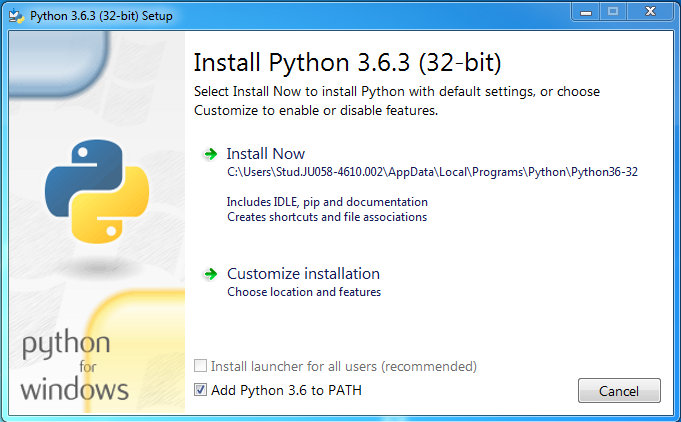
\includegraphics[scale=0.4]{images/python_install} 
    \end{figure}
\end{frame}


\begin{frame}{Entwicklungsumgebung einrichten}
    \textbf{Achtung}\\
        Word, TextEdit, Notepad, oder Wordpad sind Textverarbeitungsprogramme, keine 
        Quelltext-Editoren und schon gar keine Entwicklungsumgebungen
   
    \begin{itemize}
        \item Editoren wie \texttt{Sublime Text, Atom} oder \texttt{IDLE} sind 
         ausreichend
        \item große IDE's wie \texttt{Eclipse}, \texttt{IntelliJ} oder \texttt{PyCharm} 
        bieten weitere Funktionen
    \end{itemize}
\end{frame}

\begin{frame}{Entwicklungsumgebung einrichten}
    \begin{itemize}
        \item Pythonprogramme in IDLE schreiben und ausführen
            \begin{enumerate}
                \item\texttt{Datei} $>$ \texttt{Neue Datei}
                \item geeigneten Speicherort aussuchen, bspws. \texttt{Dokumente/GrundkursProgrammieren/helloworld.py}
                \item Programm schreiben\dots
                \item Programm unter \texttt{Run} $>$ \texttt{Run Module} ausführen oder F5 drücken
            \end{enumerate}
    \end{itemize}
\end{frame}



\begin{frame}{Weiterführendes Material}
\begin{itemize}
    \item Universität Passau: `Programmierung I' (5102) an der FIM
    \item Automate the Boring Stuff with Python: Practical Programming for Total Beginner (Sweigart, 2015)
    \item `How to think like a Computer Scientist' (Wentworth, Peter and Elkner, Jeffrey and Downey, Allen B and Meyers, Chris, 2011) 
    \item www.pythontutor.com/visualize.html
    \item https://www.w3schools.com/python/
    \item https://www.geeksforgeeks.org/python-programming-language/
\end{itemize}
\end{frame}

\begin{frame}{Evaluation}
\begin{itemize}
    \item Danke für die Teilnahme! Informationen zu weiteren Kursen im jeweiligen Semester beim ZKK
    \item \url{www.evaluation.uni-passau.de} (Unter Umständen muss noch das Zertifikat
        heruntergeladen werden)
\end{itemize}
\end{frame}



\end{document}
